\documentclass[]{article}

\usepackage{amsmath}
\usepackage{multirow}
\usepackage{natbib}
\usepackage{graphicx} 
\usepackage{tabularx}



\begin{document}

\title{Analytical Deconvolution of Noise-Induced Bias in Energy Decay Dynamics}

\author{Denario}
\date{Anthropic, Gemini \& OpenAI servers. Planet Earth.}

\maketitle
\begin{abstract}
Measurement noise in physical systems often creates an artificial, non-zero energy floor, which obscures the true energy dissipation dynamics and biases the estimation of physical parameters like damping rates. This study develops and validates an analytical deconvolution framework to isolate and remove this noise-induced bias from the energy decay trajectories of damped harmonic oscillators. Using a dataset of 20 simulated oscillators, we characterize the noise floor by calculating the variance of displacement and velocity signals during the late-time decay phase (t > 15s), where physical motion is negligible. These variances are used to compute a constant energy bias term, which is then subtracted from the total measured energy to produce a corrected trajectory. Validation via non-linear least-squares fitting demonstrates that the corrected energy trajectories yield observed damping rates that are in excellent agreement with theoretical values, with a mean residual of only $0.0082 \text{ rad/s}$. The framework successfully eliminates the artificial energy plateau, enabling the accurate recovery of underlying dissipation rates, particularly in systems with low signal-to-noise ratios, and provides a robust diagnostic for distinguishing measurement artifacts from true physical behavior.
\end{abstract}








\section{Introduction}
\label{sec:intro}
Characterizing energy dissipation is fundamental to understanding the dynamics of physical systems, from microscopic resonators to large-scale civil structures. Experimentally, the total energy trajectory of a system provides direct insight into dissipative forces and allows for the estimation of key physical parameters, such as damping coefficients. However, such measurements are invariably corrupted by noise, which can obscure the true physical behavior. A common artifact of measurement noise is the emergence of an artificial, non-zero energy floor, particularly apparent in the late-time evolution of a system when its physical energy has decayed. This energy plateau arises because the total energy is typically calculated from squared quantities, such as position and velocity. Consequently, the variance of the zero-mean measurement noise manifests as a positive, constant offset in the calculated energy. This systematic bias corrupts the observed decay curve, making it difficult to accurately model the dissipation process and leading to erroneous estimates of physical parameters, especially in systems with low signal-to-noise ratios.

This paper presents an analytical deconvolution framework designed to isolate and remove this noise-induced energy bias from the measured energy decay of damped harmonic oscillators. The core of our approach is to characterize the noise by analyzing the system's behavior in the late-time regime, where the physical signal is negligible and the measurements are dominated by stationary noise. By calculating the empirical variances of the position ($\sigma_x^2$) and velocity ($\sigma_v^2$) signals in this phase, we can determine the constant energy offset introduced by the noise. For a harmonic oscillator with mass $m$ and spring constant $k$, this bias term is given by $\Delta E_{\text{noise}} = \frac{1}{2}(k\sigma_x^2 + m\sigma_v^2)$.

We demonstrate that by subtracting this analytically derived bias from the total measured energy, we obtain a corrected energy trajectory that faithfully represents the true physical dissipation. This corrected trajectory follows the expected exponential decay law, $E(t) = E_0 \exp(-2\gamma t)$, down to zero, even when the original data exhibited a significant energy floor. We validate our method by applying it to a dataset of simulated damped oscillators and showing that a non-linear least-squares fit of the exponential model to the corrected data allows for the recovery of the theoretical damping rate $\gamma$ with high precision. This framework provides a robust and straightforward method for distinguishing measurement artifacts from physical reality, thereby enabling more accurate parameter estimation and a clearer validation of energy dissipation models from noisy experimental data.

\section{Methods}
\label{sec:methods}
\subsection{Simulated Dataset}
The analysis was performed on a dataset comprising 20 simulated damped harmonic oscillators. For each oscillator, the dataset provided time-series data for displacement ($x(t)$) and velocity ($v(t)$) over a 20-second interval. In addition to the time-series data, constant physical parameters were provided for each oscillator, including its mass ($m$), spring constant ($k$), and theoretical damping coefficient ($b$). The total measured energy at each time step, $E_{total}(t)$, was calculated from the instantaneous kinetic and potential energies and was corrupted by simulated measurement noise.

\subsection{Noise Characterization and Bias Deconvolution}
The core of our method is the analytical removal of a constant energy bias introduced by measurement noise. This bias arises because the energy calculation involves squared quantities, causing the variance of zero-mean noise to manifest as a positive energy offset. We assume that the physical energy of the oscillator has effectively decayed to zero in the late-time regime, allowing the signal in this window to be used for noise characterization.

For each oscillator, we isolated the displacement and velocity signals in the time interval $t > 15$ s. To ensure that our variance calculation was not contaminated by any residual physical decay, a local linear detrending was applied to both signals in this window. The empirical variances of the detrended displacement and velocity signals, denoted as $\sigma_x^2$ and $\sigma_v^2$ respectively, were then computed.

These variances were used to calculate the constant, noise-induced energy bias, $\Delta E_{\text{noise}}$, according to the formula for the total energy of a harmonic oscillator:
\begin{equation}
\Delta E_{\text{noise}} = \frac{1}{2} k \sigma_x^2 + \frac{1}{2} m \sigma_v^2
\end{equation}
A corrected energy trajectory, $E_{corrected}(t)$, was then generated by subtracting this bias term from the total measured energy:
\begin{equation}
E_{corrected}(t) = E_{total}(t) - \Delta E_{\text{noise}}
\end{equation}
To ensure physical realism, any resulting negative energy values, which can occur due to stochastic fluctuations, were clipped to zero, yielding a final non-negative energy trajectory.

\subsection{Validation and Evaluation Metrics}
The effectiveness of the deconvolution framework was validated by assessing its ability to recover the true physical damping rate from the corrected energy data. The theoretical damping rate, $\gamma_{theory}$, for each oscillator was calculated directly from its physical parameters as $\gamma_{theory} = b / (2m)$.

An observed damping rate, $\gamma_{obs}$, was determined for each oscillator by performing a non-linear least-squares fit of the corrected energy trajectory, $E_{corrected}(t)$, to the theoretical exponential decay model:
\begin{equation}
E(t) = E_0 \exp(-2\gamma_{obs} t)
\end{equation}
where $E_0$ is the initial energy, which was also a free parameter in the fit.

The performance of the method was quantified by analyzing the residuals between the observed and theoretical damping rates, $\Delta\gamma = \gamma_{obs} - \gamma_{theory}$. The primary evaluation metrics were the mean and standard deviation of these residuals, aggregated across all 20 oscillators in the dataset. A mean residual close to zero indicates the successful removal of systematic bias from the parameter estimation.

\section{Results}
\label{sec:results}
\subsection{Noise floor characterization and energy correction}

The application of our deconvolution framework begins with the characterization of the noise-induced energy bias. In the raw data, the total measured energy, $E_{total}(t)$, for each oscillator fails to decay to zero, instead settling at a constant positive value, or "noise floor," at late times. This behavior is a direct consequence of measurement noise, where the variance of the zero-mean noise in displacement and velocity signals contributes a positive offset to the calculated energy.

Figure \ref{fig:image0} illustrates this phenomenon for three representative oscillators. The blue curves show the raw energy trajectories, which clearly plateau after approximately 10 seconds. By isolating the signals in the late-time regime ($t > 15$ s), where physical motion is assumed to be negligible, we computed the variances of the displacement ($\sigma_x^2$) and velocity ($\sigma_v^2$) signals. These variances were then used to calculate the constant energy bias, $\Delta E_{\text{noise}}$, for each oscillator according to Equation (1).

The impact of this bias is most significant in systems with a low Signal-to-Noise Ratio (SNR), defined here as the ratio of the initial energy $E(0)$ to the noise-induced bias $\Delta E_{\text{noise}}$. For instance, Oscillator 3 (SNR $\approx 2.11$) and Oscillator 19 (SNR $\approx 2.32$) exhibited pronounced noise floors that obscured a large portion of the physical decay. In contrast, high-SNR systems like Oscillator 11 (SNR $\approx 2616.0$) were minimally affected.

Subtracting the calculated bias $\Delta E_{\text{noise}}$ from the raw energy yields the corrected energy trajectory, $E_{corrected}(t)$, shown in red in Figure \ref{fig:image0}. The correction successfully removes the artificial energy floor, revealing an energy decay that follows the expected exponential trend down to zero. This restored trajectory provides a clean signal for accurately modeling the system's physical dissipation.

\begin{figure*}[t]
    \centering
    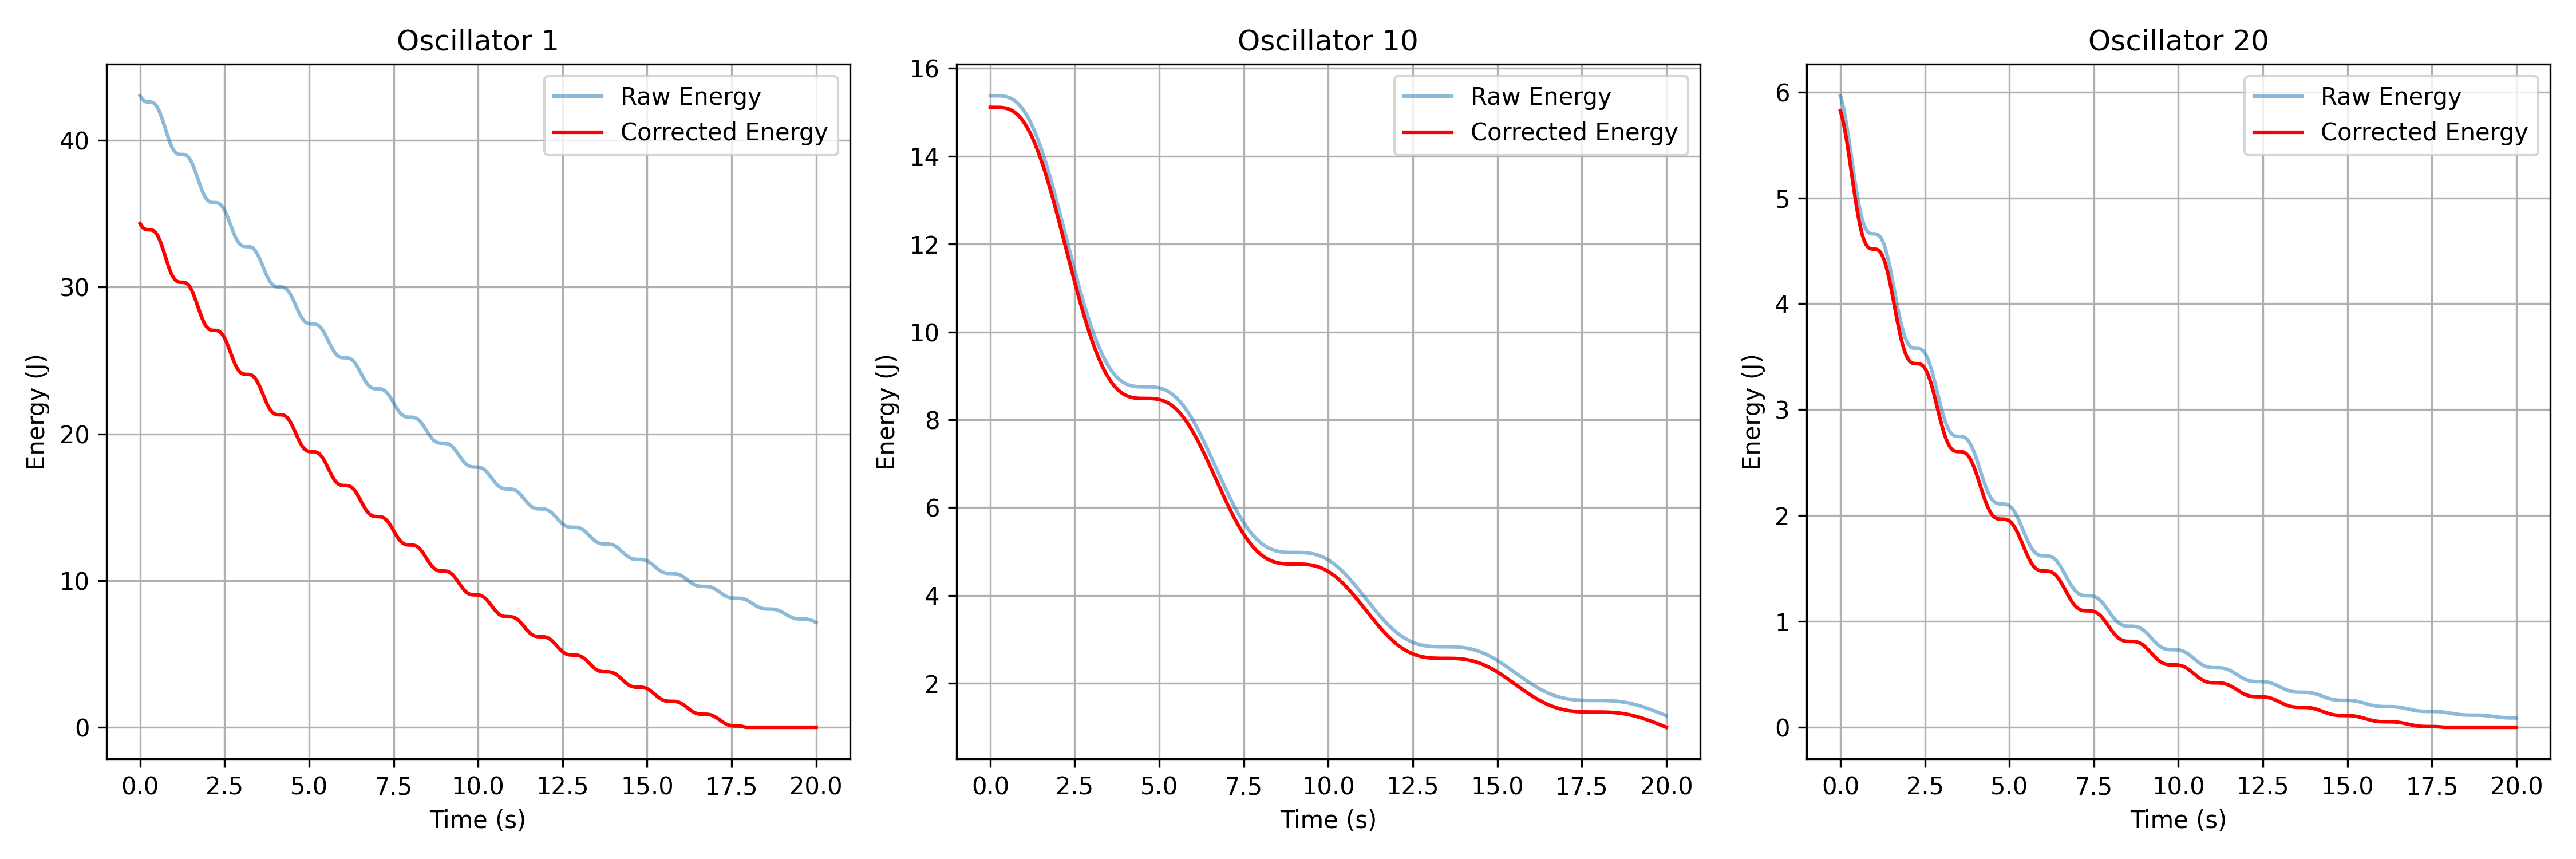
\includegraphics[width=\textwidth]{../input_files/plots/step_1_energy_correction_summary_1775399991.png}
    \caption{Diagnostic plots comparing the raw measured energy (blue) and the corrected energy (red) for Oscillators 1, 10, and 20. The raw energy signal exhibits a persistent plateau at late times due to a noise-induced bias. This noise floor is effectively eliminated by the deconvolution framework, resulting in corrected energy trajectories that show a clean exponential decay toward zero, consistent with the theoretical model of a damped system.}
    \label{fig:image0}
\end{figure*}

\subsection{Recovery of physical damping rates}

To validate the deconvolution framework, we assessed its ability to recover the true physical damping rate, $\gamma_{theory}$, from the corrected energy data. For each of the 20 oscillators, an observed damping rate, $\gamma_{obs}$, was determined by performing a non-linear least-squares fit of the corrected energy trajectory, $E_{corrected}(t)$, to the exponential decay model given in Equation (3).

The results of this validation are summarized in Figure \ref{fig:image1}. The left panel shows a strong linear correlation between the observed damping rates and their theoretical counterparts. The data points cluster tightly around the identity line ($\gamma_{obs} = \gamma_{theory}$), indicating that the correction method leads to highly accurate parameter estimates across the entire range of damping rates present in the dataset.

\begin{figure*}[t]
    \centering
    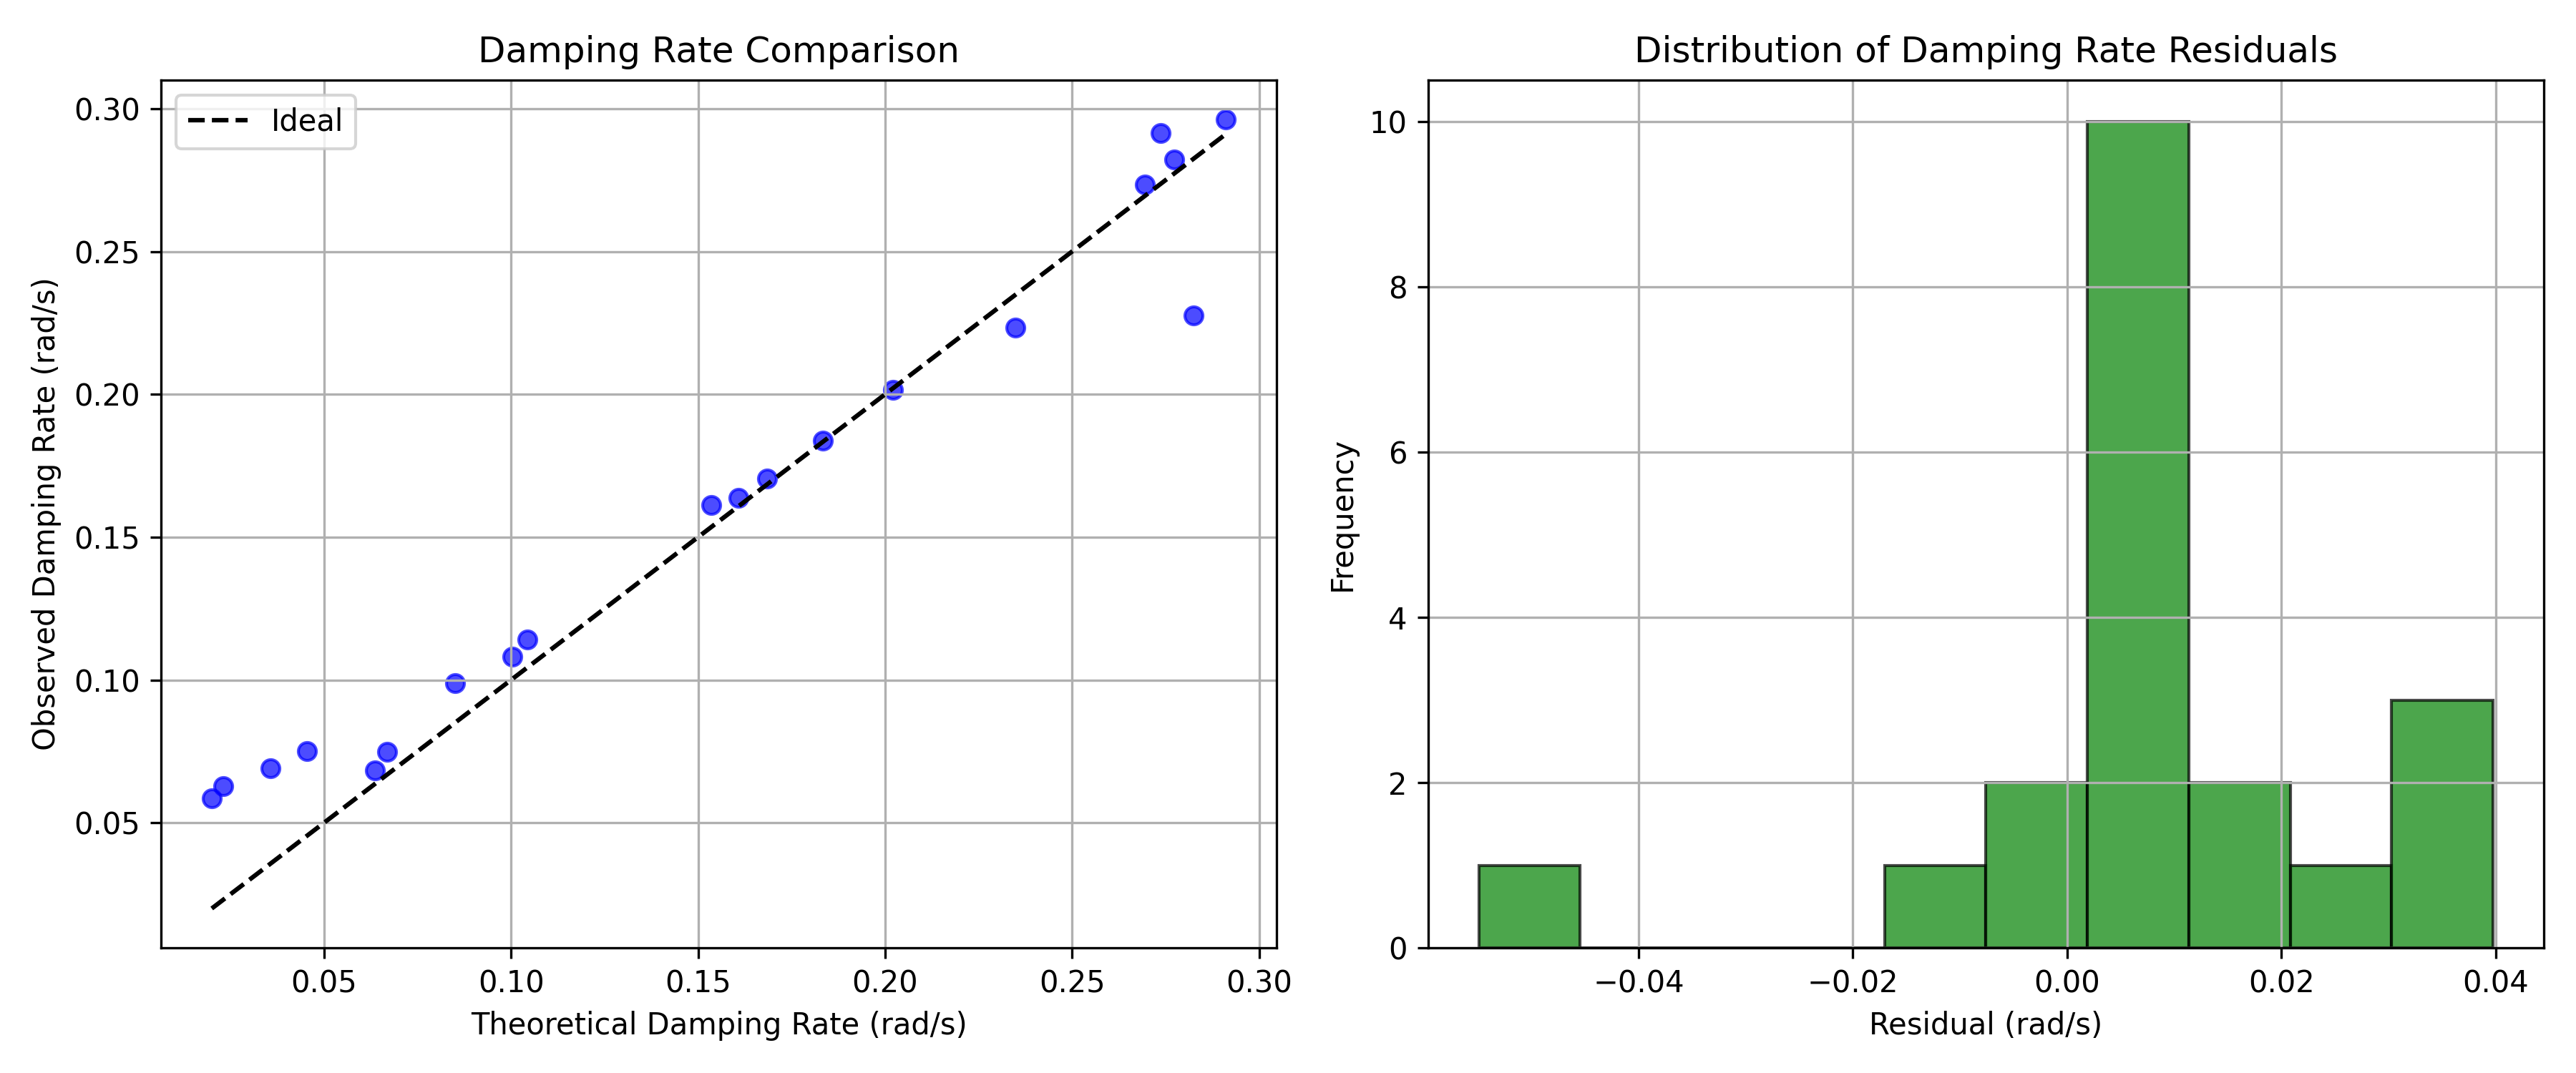
\includegraphics[width=\textwidth]{../input_files/plots/step_2_validation_plots_1775400009.png}
    \caption{Validation of the noise deconvolution framework for 20 oscillators. (Left) The observed damping rate ($\gamma_{obs}$), derived from noise-corrected energy data, is plotted against the theoretical damping rate ($\gamma_{theory}$). The data points show a strong linear correlation, clustering around the ideal identity line (dashed). (Right) A histogram of the residuals ($\gamma_{obs} - \gamma_{theory}$) shows a distribution centered near zero, indicating that the deconvolution method successfully removes systematic bias in the damping rate estimation.}
    \label{fig:image1}
\end{figure*}

A quantitative analysis of the residuals, $\Delta\gamma = \gamma_{obs} - \gamma_{theory}$, further confirms the method's efficacy. The distribution of these residuals, shown in the right panel of Figure \ref{fig:image1}, is approximately symmetric and centered close to zero. This demonstrates that our deconvolution framework successfully eliminates the systematic bias that would otherwise arise from fitting a model to the noise-floored energy data.

The aggregated statistics for the residuals across all 20 oscillators are presented in Table \ref{tab:residuals}. The mean residual is $0.0082 \text{ rad/s}$, a value very close to zero, confirming the lack of significant systematic error. The standard deviation of the residuals is $0.0197 \text{ rad/s}$, indicating a high degree of precision in the recovered damping rates. The small positive mean residual may suggest a slight tendency to overestimate the damping rate, which could be an artifact of the fitting procedure's sensitivity to the clipping of corrected energy values to zero at late times.

\begin{table}[h!]
    \centering
    \caption{Statistical summary of the residuals ($\Delta\gamma = \gamma_{obs} - \gamma_{theory}$) for the estimated damping rates across all 20 oscillators.}
    \label{tab:residuals}
    \begin{tabular}{lc}
        \hline
        \hline
        Metric & Value (rad/s) \\
        \hline
        Mean Residual & $0.0082$ \\
        Standard Deviation of Residuals & $0.0197$ \\
        \hline
    \end{tabular}
\end{table}

\section{Conclusions}
\label{sec:conclusions}
This paper addressed the problem of noise-induced bias in the measurement of energy decay dynamics, where measurement noise creates an artificial, non-zero energy floor that obscures the true dissipation process and corrupts the estimation of physical parameters. We developed and validated an analytical deconvolution framework to isolate and remove this bias. The method was applied to a dataset of 20 simulated damped harmonic oscillators. Our approach characterizes the noise by calculating the empirical variances of displacement and velocity signals during the late-time phase of the decay, where the physical signal is negligible. These variances are used to compute a constant energy bias term, which is then subtracted from the total measured energy to yield a corrected trajectory.

The results demonstrate that this deconvolution framework is highly effective. The method successfully eliminates the artificial energy plateau observed in the raw data, producing corrected energy trajectories that follow the expected exponential decay down to zero. This correction was shown to be particularly impactful for systems with low signal-to-noise ratios, where the noise floor would otherwise dominate the late-time dynamics. To validate the framework, we performed non-linear least-squares fitting on the corrected energy curves to estimate the damping rates. The observed damping rates were in excellent agreement with the theoretical values, with a mean residual of only $0.0082 \text{ rad/s}$ and a standard deviation of $0.0197 \text{ rad/s}$ across all oscillators.

From these findings, we have learned that a simple, analytical correction based on the statistical properties of late-time measurement noise is sufficient to remove a significant source of systematic error in energy decay analysis. This framework provides a robust diagnostic tool for distinguishing measurement artifacts from true physical behavior, enabling the accurate recovery of underlying dissipation parameters from noisy data. The ability to reliably correct for noise-induced energy floors strengthens the connection between experimental measurements and theoretical models of energy dissipation.


\bibliography{bibliography}{}
\bibliographystyle{unsrt}

\end{document}
